
\setcounter{section}{0}
\setcounter{figure}{0}
\graphicspath{{./figs/}{./figs/item-rajiv/}}

\NewsTitle{End-to-End QoS Specification and Monitoring in the Internet of Things}
\NewsAuthor{Awatif Alqahtani$^1$, Ellis Solaiman$^1$, Rajkumar Buyya$^2$, Rajiv Ranjan$^1$\\
$^1$School of Computing Science, Newcastle University, United Kingdom \\
$^2$Computing and Information Systems, University of Melbourne, Australia}

The Internet of Things (IoT) is a computing paradigm where uniquely addressable objects such as Radio-Frequency IDentification (RFID) tags, sensors, actuators, and mobile phones, are able to connect via the Internet, and cooperate with each other in order to achieve common goals \cite{ref1,ref4}.
The number of connected smart objects is estimated to reach 212 billion by the end of 2020 \cite{ref2,ref3}.
Such large numbers of connected smart objects will generate huge volumes of data that needs to be analysed and stored \cite{ref6}.
According to a study conducted by IBM, 2.5 quintillion bytes of data is generated every day \cite{ref7}.
Storing and processing such large volumes of Big Data is non-trivial, and requires the flexibility offered by Cloud Computing \cite{ref8}.
Cloud Computing offers a pool of configurable resources (hardware/software) that are available on demand \cite{ref9},
allowing users to submit jobs to service providers on the basis of pay-per-use.
While the IoT provides smart devices with the ability to sense and generate large amount of data that reflect the physical world in different forms and different data speeds,
Cloud Computing offers advanced technologies for ingesting, analysing and storing data \cite{ref10}.
The number of applications based on IoT and Cloud Computing is projected to increase rapidly over next few years.
To this end, Gascon and Asin \cite{ref11} predicted that in near future there will be about 54 types of IoT applications for addressing different domain \cite{ref5} specific problems: security and emergency, smart environment, smart cities, smart metering, smart water, smart animal farming, smart agriculture, industrial control, retail, logistics, domestic and home automation and e-Health. 

\section{Quality of Service roadmap for IoT applications}

Expectation from services provided by the Internet of Things are no different from most traditional computer and Internet based services in that they must be delivered with guaranteed levels of quality of service (QoS).
For example, in emergency response (ER) IoT application, there is a need to receive and analyse data from deployed sensors immediately and accurately in order to allow for timely response to potential damage that can be caused in natural disaster situations such as earthquakes, floods, and tsunamis \cite{ref12}.
Such IoT applications can be extremely time sensitive; any delay in the collection/transferring/ingestion/analysis of sensor data may have disastrous consequences.

As we note in our previous papers \cite{ref4,ref13}, engineering IoT applications that can guarantee QoS is a challenging and not feasible with the current state-of-the-art available in context of IoT programming models (e.g. Amazon IoT, Google Cloud Dataflow, IBM Quark) and resource management methods \cite{ref4,ref33}.
An important difficulty is that IoT application eco-systems are typically consists of several layers involving multiple, heterogeneous hardware and software resources;
and data types from digital and human sensors. An example of an IoT eco-system is depicted in Figure \ref{fig:1},
which consists of following programming and resource management layers; sensing layer, gateway layer, network layer, and cloud layer.
Providing customers with QoS guarantees requires the technical ability to ensure that their QoS requirements will be observed across each of the layers of an IoT application eco-system.

\begin{figure}[h]
    \centering
    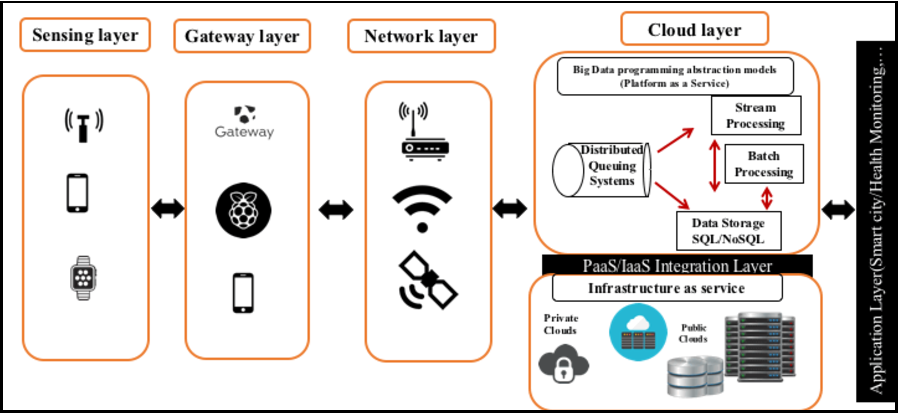
\includegraphics[width=.68\textwidth]{fig1}
    \caption{A multi-layered architecture IoT application eco-system involving Sensing, Gateway, Network, and Cloud layers.}
    \label{fig:1}
\end{figure}

\section{Specification of IoT application specific QoS requirements within Service Level Agreements}

In purely business context, QoS requirements are formally specified in a Service Level Agreement (SLA) document \cite{ref3} which serves as the basis of legal agreement and understanding of service terms, conditions, and commitments between consumers and providers.
For example, Amazon Web Services' SLA document stating the terms, conditions, and commitments for its S3 and EC2 services can be found at \cite{ref34} and \cite{ref35} respectively.

As IoT applications have layered architecture and complex Big Data flows across layers, there is a need to first model SLA for individual layers followed by their holistic aggregation.
Such aggregated SLA document (template) will form basis for specifying an end-to-end SLA that can be used to specify the service terms,
conditions and commitments for an IoT application. Notably, cross-layer SLAs in IoT have a strong dependency relationships with each of its upstream and downstream layers,
regardless of whether this component is data, computing hardware, IoT sensor, software, or human.
Thus violation of one or more constraints by one or more components (s) affects the adherence to the related SLA's terms. 

To illustrate this concept, consider a remote health monitoring IoT application \cite{ref13} where patients wear sensors and accelerometers to measure their heart rate and sugar levels, reminding them of the time to take medications, and detecting abnormal activities such as falling down.
Subscribed patients might ask for a service that can satisfy the following high-level, strict SLA requirement: detecting abnormal activity, such as falling down, within x milliseconds, then alerting/notifying the ambulance, caregivers, and doctors within y minutes.
To achieve this high-level SLA requirement, many nested-dependent QoS metrics should be considered, such as high-quality sensors with minimum event detection delay (within x milliseconds), available networks with low latency, and a high-alert detection and notification analytic service to deliver the desirable alerts to relevant healthcare providers and relatives.
As patients need to receive the required emergency treatment based on their health status within y minutes, this means that the aggregation of the response time from each layer should be within the time constraints, i.e.~less than or equal to y minutes.
A delay in the network, for example, would lead to a late response at the alert generation front-end, which could exceed the time the patient and healthcare provider was expecting (y minutes).
Specifying SLA requirements with their required level of QoS and monitoring their adherence to these specifications is a non-trivial task and includes many challenges such as:
\begin{description}
  \item[A.] Heterogeneity of Big Data sources and their distributed locations.
  \item[B.] Heterogeneity of the key QoS metrics across layers.
  \item[C.] Heterogeneity of application requirements.
  \item[D.] Lack of unified/standard methods for collecting the required metrics across-layer and from multiple providers for end-to-end SLA monitoring purposes.
\end{description}

\section{SLA specification and monitoring current research efforts:}

Substantial research on the specification and monitoring of QoS and SLAs has been conducted for computer networks, web services, Grids, and Cloud Computing.
But limited literature is available that deal the problem of specifying and monitoring end-to-end QoS and SLAs in an IoT application eco-system.
For example, Netlogger provides an API that can be used by applications to check the load on network resources before and after performing operations / sending requests.
However, Netlogger only monitors network resources and does not extend to other components of an IoT application \cite{ref14,ref15}.
The Web Service Level Agreement (WSLA) standard described in \cite{ref16} was developed for web service SLA specification.
Also, WS-Agreement from the Open Grid Forum (OGF) defines a web service agreement specification as a protocol for launching an agreement between two parties.
An illustration of how cloud providers in industry apply SLAs is shown in \cite{ref21}.
Cloud providers such as AmazonEC2, S3 (IaaS provider) and Windows Azure Compute and Storage, serve a pre-defined SLA, and the user can then choose the most appropriate provider that will fit their requirements.
After entering into a contract with the selected provider, the SLA can be monitored against violations using third parties such as Cloudwatch, Cloudstatus and Monitis.
The LoM2HiS Framework \cite{ref14} aims to monitor and enforce SLA objectives in the cloud environment, especially; scalability, efficiency and reliability requirements.
The framework aims to map low-level resource metrics to high SLAs objectives.
However, the LoM2HiS Framework does not extend beyond the Cloud infrastructure layer.
A European Commission Report on Cloud Computing Service Level Agreements \cite{ref24} identifies and describes several interesting research efforts.
SLA(T) by the SLA@SOI project \cite{ref25,ref27} is a model and language for service description that expresses the dependencies among services within / across layers in the Cloud. Another project (CONTRAIL) provides a quality model \cite{ref28} for capturing different parameters of interest for customers and providers.
The IRMOS project \cite{ref3} proposes two SLAs at different levels: an application SLA to express high-level application terms between consumers and providers, and technical SLAs to express the low level QoS parameters linked to the infrastructure resources.
Cloud4SOA \cite{ref31}, is a project which provides a unified monitoring interface that gives an overview of all of the customer deployments at one time, as well as selecting a set of unified metrics for monitoring both the execution and the usage of an application.
IRMOS \cite{ref32} provides an adaptable monitoring framework that collects data from both the application and technical level to monitor real-time application execution at time intervals based on the collected monitoring information and its associated SLA terms. 

Despite a number of impressive research efforts into the specification and monitoring of QoS requirements within networks, web services, grids, and clouds, none of these are suitable in context of IoT applications.
Developing formal approaches for the specification of QoS requirements and monitoring end-to-end IoT ecosystems is what we term as the next ``grand challenge'' for distributed systems researchers,
and current platforms and techniques for monitoring IoT and Cloud computing fall short of this grand challenge.


\begin{thebibliography}{10}

\bibitem{ref1}
A.~Flammini, and E.~Sisinni.
\newblock {Wireless Sensor Networking in the Internet of Things and Cloud Computing Era}.
\newblock {\em Procedia Engineering}, vol.~87, pp.~672--679, Dec.~2014.

\bibitem{ref2}
J.~Gantz and D.~Reinsel.
\newblock {The digital universe in 2020: Big data, bigger digital shadows, and biggest growth in the Far East}.
\newblock {\em IDC iView: IDC Anal. Future}, vol.~2007, pp.1--16, Dec.~2012.

\bibitem{ref3}
A.~Galati et al.
\newblock {A WS-Agreement based SLA implementation for the CMAC platform}.
\newblock In {\em Economics of Grids, Clouds, Systems, and Services}, Springer-Verlag Heidelberg: Springer International Publishing, 2014. 

\bibitem{ref4}
R.~Ranjan.
\newblock {Streaming big data processing in datacenter clouds}.
\newblock {\em IEEE Cloud Computing}, vol.~1, no.~1, pp.78--83, May 2014.

\bibitem{ref5}
R.~Buyya, and A.V.~Dastjerdi, eds.
\newblock {Internet of Things: Principles and Paradigms}, Elsevier, 2016.

\bibitem{ref6}
K.~Radha et al.
\newblock {Service Level Agreements in Cloud Computing and Big Data}.
\newblock {\em International Journal of Electrical and Computer Engineering}, 5(1), p.158, Feb.~2015. 

\bibitem{ref7}
\newblock {IBM What is Big Data? -- Bringing Big Data to the Enterprise}.
\newblock \url{https://www-01.ibm.com/software/data/bigdata/what-is-big-data.html}

\bibitem{ref8}
Zheng, X., Martin, P., Brohman, K. and Da Xu, L.
\newblock {Cloud service negotiation in internet of things environment: a mixed approach}.
\newblock {\em Industrial Informatics, IEEE Transactions on}, vol.~10, pp.~1506-1515, May 2014.

\bibitem{ref9}
M.~D{\'\i}az, C.~Mart{\'\i}n, and B.~Rubio.
\newblock {State-of-the-art, challenges, and open issues in the integration of Internet of things and cloud computing}.
\newblock {\em Journal of Network and Computer Applications}, 2016.

\bibitem{ref10}
M.~Chen, S.~Mao, and Y.~Liu.
\newblock {Big data: a survey}.
\newblock {\em Mobile Networks and Applications}, vol.~19, no.~2, pp.171--209, Apr.~2014.

\bibitem{ref11}
D.~Gascon, and A.~Asin.
\newblock {50 sensor applications for a smarter world}.
\newblock \url{http://www.libelium.com/resources/top_50_iot_sensor_applications_ranking}, 2015

\bibitem{ref12}
N.~Li et al.
\newblock {A new methodology to support group decision-making for IoT-based emergency response systems}.
\newblock {\em Information Systems Frontiers}, vol.16, no.5, pp.953--977, 2014.

\bibitem{ref13}
P.P.~Jayaraman et al.
\newblock {Orchestrating Quality of Service in the Cloud of Things Ecosystem}.
\newblock In {\em IEEE International Symposium on Nanoelectronic and Information Systems}, pp.185--190, December 2015.

\bibitem{ref14}
V.C.~Emeakaroha et al.
\newblock {Low level metrics to high level SLAs-LoM2HiS framework: Bridging the gap between monitored metrics and SLA parameters in cloud environments}.
\newblock In {\em International Conference High Performance Computing and Simulation (HPCS)}, pp.~48--54), June 2010.

\bibitem{ref15}
D.~Gunter et al.
\newblock {Netlogger: a toolkit for distributed system performance analysis}.
\newblock {\em International Symposium on Modeling, Analysis and Simulation of Computer and Telecommunication Systems}, pp.~267--273, 2000.

\bibitem{ref16}
A.~Keller, and H.~Ludwig.
\newblock {The WSLA framework: Specifying and monitoring service level agreements for web services}.
\newblock {\em Journal of Network and Systems Management}, vol.~11, no.~1, pp.57--81, Mar 2003.

\bibitem{ref17}
M.~Alhamad, T.~Dillon, and E.~Chang.
\newblock {Service level agreement for distributed services: a review}.
\newblock In {\em IEEE International Conference on Dependable, Autonomic and Secure Computing (DASC)}, pp.~1051--1054), Dec.~2011.

\bibitem{ref18}
A.~Andrieux et al.
\newblock {Web services agreement specification (WS-Agreement)}.
\newblock In {\em Open Grid Forum}, vol.~128, no.~1, p.~216, Mar, 2007.

\bibitem{ref19}
A.~Sahai et al.
\newblock {Specifying and monitoring guarantees in commercial grids through SLA}.
\newblock In {\em Cluster Computing and the Grid}, 2003.

\bibitem{ref20}
M.~Alhamad, T.~Dillon, and E.~Chang.
\newblock {A survey on SLA and performance measurement in cloud computing}.
\newblock In {\em On the Move to Meaningful Internet Systems: OTM}, pp.~469--477), Springer Berlin Heidelberg, 2011.

\bibitem{ref21}
L.~Wu, and R.~Buyya.
\newblock {Service Level Agreement (SLA) in utility computing systems}.
\newblock {\em IGI Global}, Apr.~2012.

\bibitem{ref22}
K.~Alhamazani et al.
\newblock {Cross-Layer Multi-Cloud Real-Time Application QoS Monitoring and Benchmarking As-a-Service Framework}.
2015.

\bibitem{ref23}
G.~Cicotti et al.
\newblock {How to monitor QoS in cloud infrastructures: The QoSMONaaS approach}.
\newblock In {\em Intelligent Distributed Computing VI}, pp.~253--262), Springer Berlin Heidelberg, 2013.

\bibitem{ref24}
D.~Kyriazis.
\newblock {Cloud computing service level agreements: exploitation of research results}.
\newblock {\em European Commission Directorate General Communications Networks Content and Technology Unit}, Tech.~Rep, 2013.

\bibitem{ref25}
SLA@SOI Project.
\newblock \url{http://sla-at-soi.eu/}

\bibitem{ref26}
RESERVOIR Project.
\newblock \url{http://www.reservoir-fp7.eu/}

\bibitem{ref27}
4CaaSt Project.
\newblock \url{http://4caast.morfeo-project.org/}

\bibitem{ref28}
R.~Cascella et al.
\newblock {Contrail: Distributed Application Deployment under SLA in Federated Heterogeneous Clouds}.
Springer, Lecture Notes in Computer Science, 2013.

\bibitem{ref29}
Q-ImPrESS Consortium.
\newblock {Service Architecture Meta-Model (SAMM)}.
\newblock {Project deliverable d2.1, Sep. 2008}.
Available: \url{http://www.q- impress.eu/wordpress/wp-content/uploads/2009/05/d21-service_architecture_meta-model.pdf}

\bibitem{ref30}
\newblock \url{http://irmosproject.eu/Files/IRMOS_NEXOF-RA_SLAs_QoS.pdf}

\bibitem{ref31}
Cloud4SOA Project.
\newblock \url{http://www.cloud4soa.eu/}

\bibitem{ref32}
IRMOS Project.
\newblock \url{http://www.irmosproject.eu/}

\bibitem{ref33}
L.~Wang and R.~Ranjan.
\newblock {Processing Distributed Internet of Things Data in Clouds}.
\newblock {\em IEEE Cloud Computing}, vol.~1, no.2, 2015.

\bibitem{ref34}
S3 SLA, Amazon Web Services.
\newblock \url{https://aws.amazon.com/s3/sla/}

\bibitem{ref35}
EC2 SLA, Amazon Web Services.
\newblock \url{https://aws.amazon.com/ec2/sla/}

\end{thebibliography}


